When working on a pack, I make tons of sketches and drawings. I start with the basic shape, I add the features I have in mind, I draw multiple mock-ups and variants of that shape, together with its prominent features. Then, I slowly focus on the details, looking at every features, each getting variants of their own. And so on, until I get a pretty good idea of what I want to build.

\index{sketch}
\begin{figure}[H]
  \includegraphics[width=\textwidth]{media/images/design-drawings-1}
  \caption{Example of drawing process (page one)}
  \label{img:design-drawings-1}
\end{figure}

In the sketches from illustration \ref{img:design-drawings-1} and \ref{img:design-drawings-2}, you can see the concept I put together before even starting working on the pack from the picture \ref{img:pack-front-full-intro}. It might not seem like a lot, but it's because I've been sketching similarly built packs for a while, and I used previous sketches, packs and mock-ups as the base for this one. I also put together a collection of images of similar packs and detailed shots of features I was going for, which complement these sketches a lot.

\index{sketch}
\begin{figure}[H]
  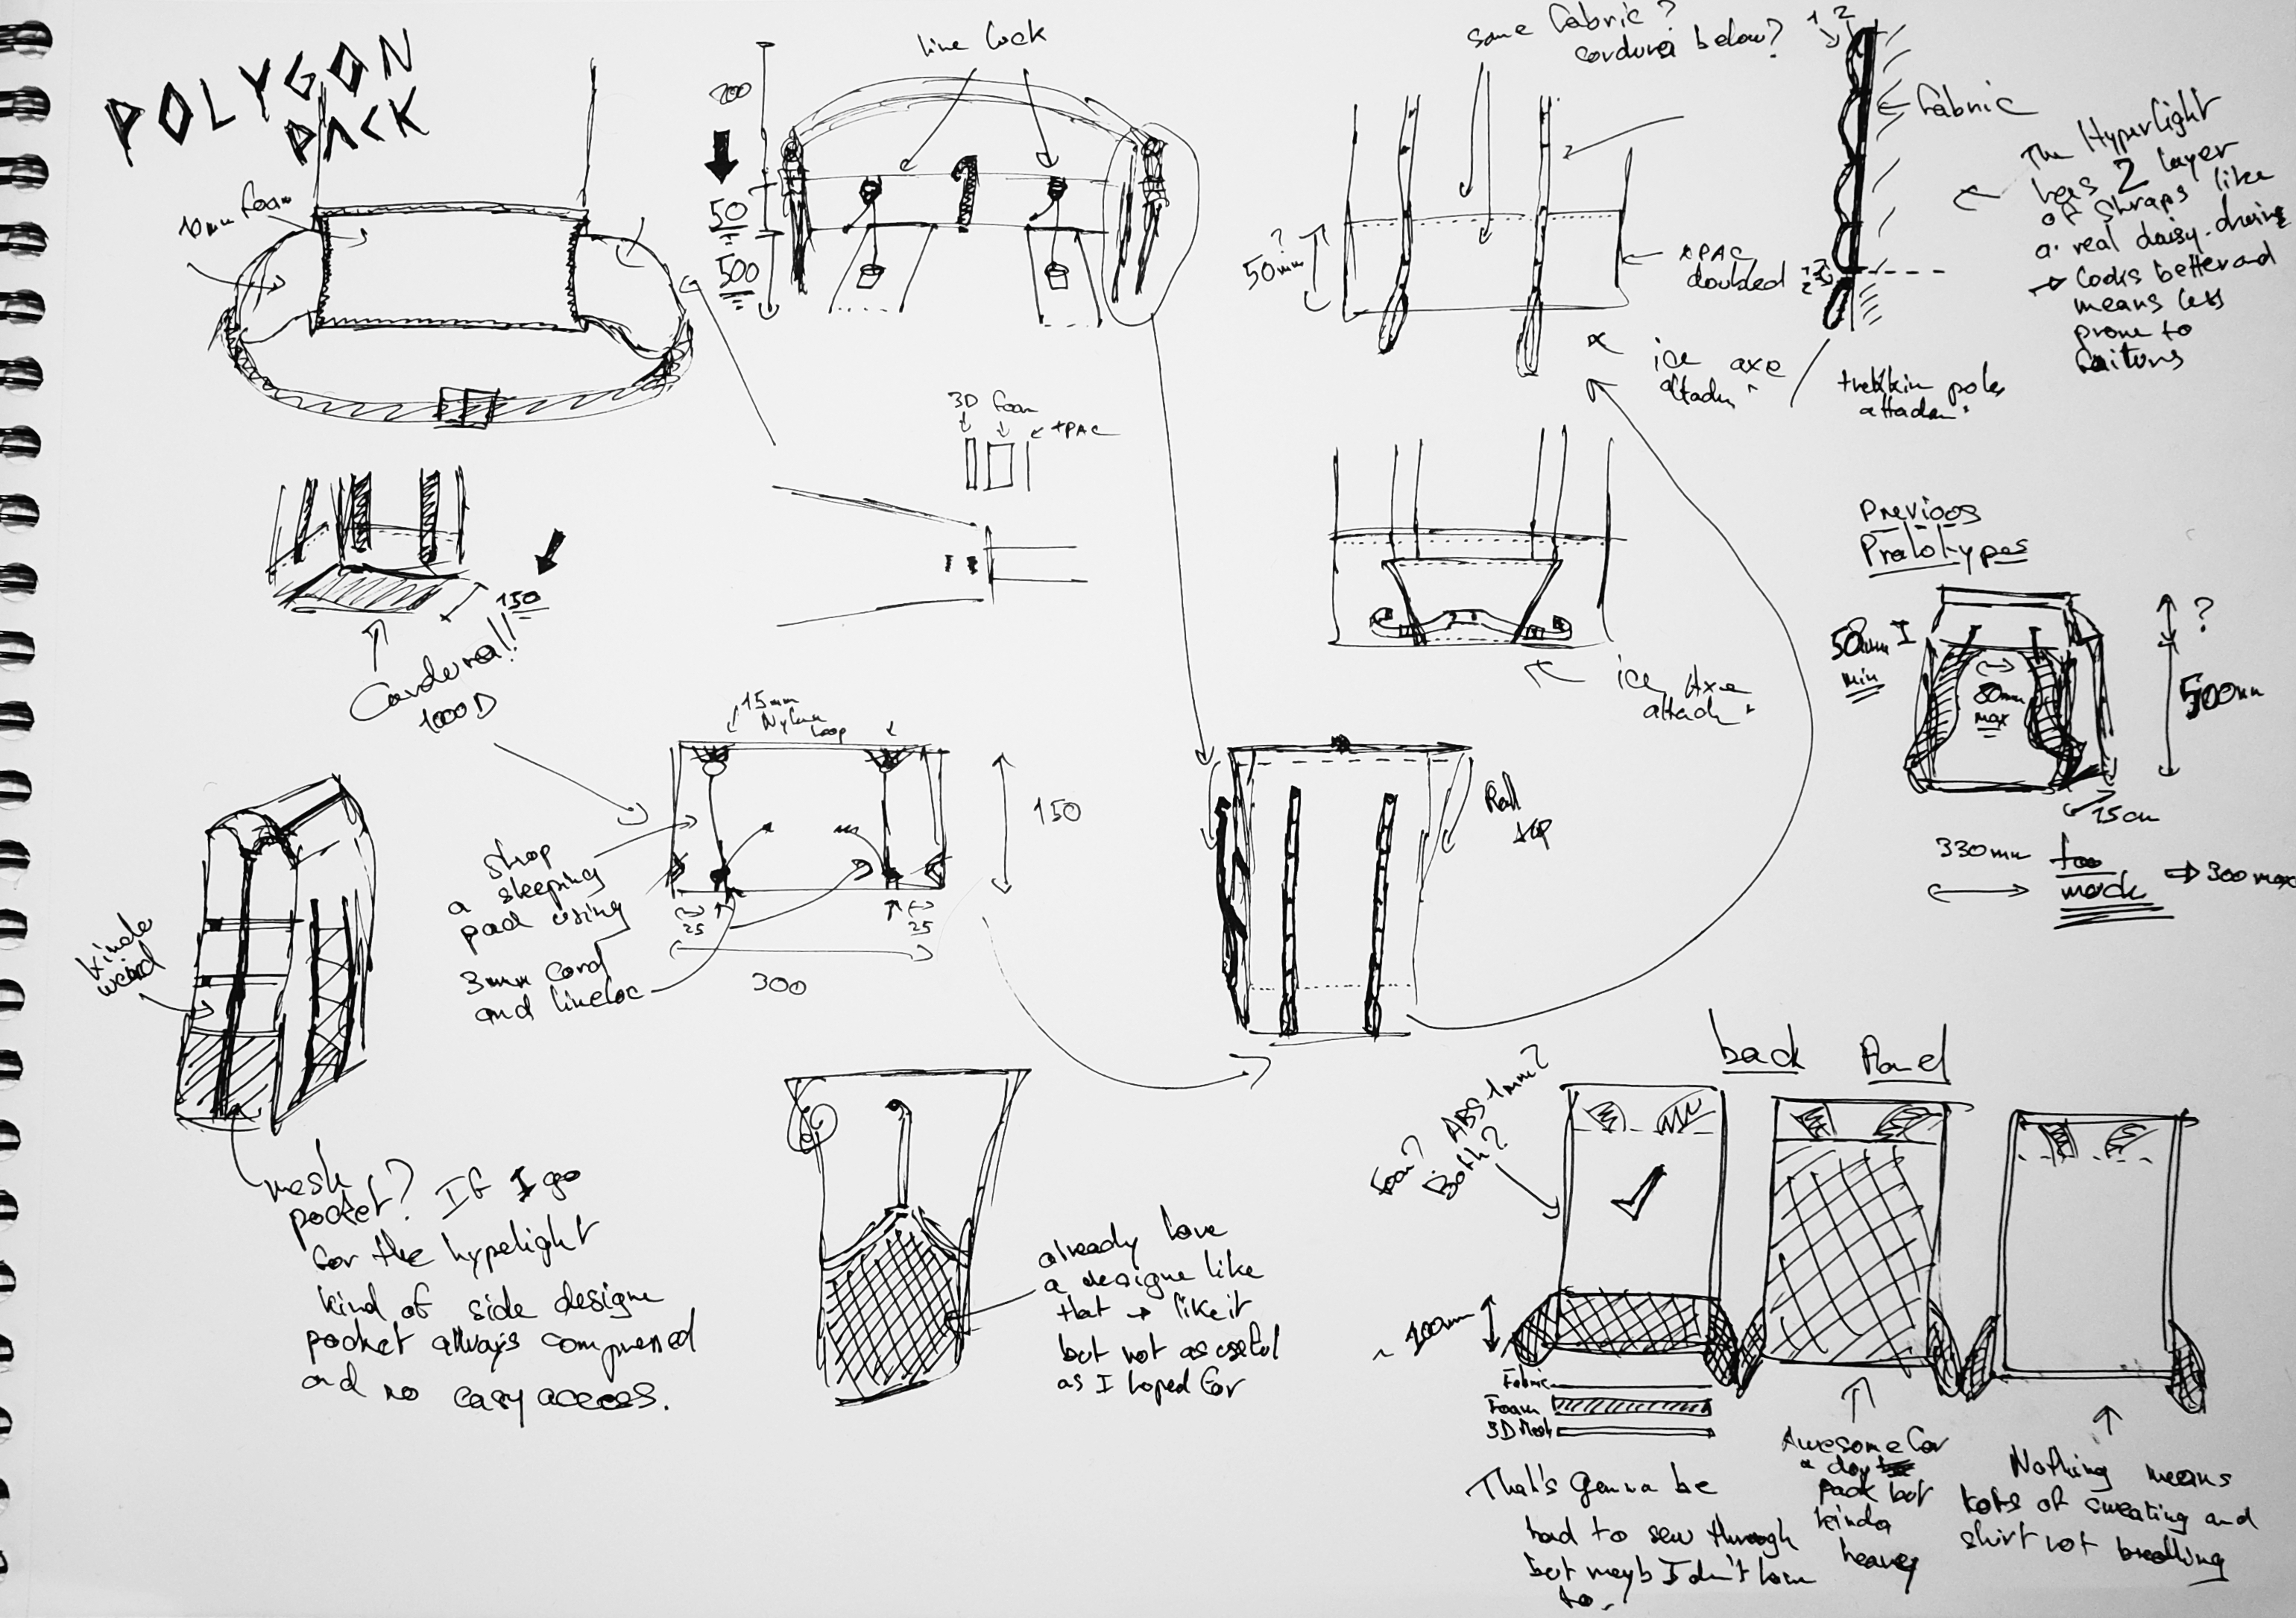
\includegraphics[width=\textwidth]{media/images/design-drawings-2}
  \caption{Example of drawing process (page two)}
  \label{img:design-drawings-2}
\end{figure}

\index{feature}
\index{pocket}
\index{shock cord}
\index{compression strap}
\index{hip-belt}
\index{padding}
For me, it's important that I highlight the features I want to add beforehand. For this pack, I knew it would have no external pockets, and instead use a front interlaced elastic shock cord for drying stuff while walking or tucking away some piece of clothing quickly. I also wanted to add a series of straps on each side of the pack for attachment and compression which I could use to strap trekking poles or a water bottle holder. On top of that, I often add a set of attachment on the bottom of the pack which can hold a closed cell foam sleeping pad (important detail, as it tells me the dimensions). In the end, I want to use that pack for loads around 5-7 kg, so a hip belt will be a must, and I might need to have the possibility to add foam padding for my back depending on what I carry.

\begin{figure}[H]
  \centering
  \includegraphics[width=\textwidth]{media/images/pack-front-full}
  \caption{The end result of the example design in illustration \ref{img:design-drawings-1}}
  \label{img:pack-front-full-intro}
\end{figure}
